\documentclass[border=5pt,tikz]{standalone}
\usetikzlibrary{arrows.meta,automata,positioning}

\begin{document}
    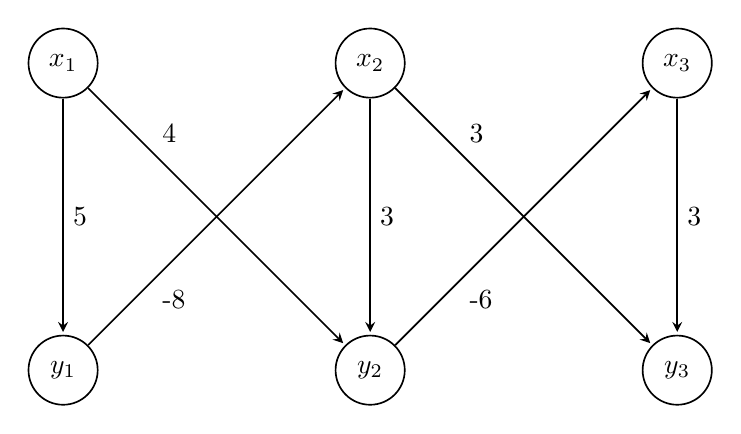
\begin{tikzpicture}[
    > = stealth, % arrow head style
    shorten > = 1pt, % don't touch arrow head to node
    auto,
    node distance = 3cm, % distance between nodes
    semithick % line style
    ]

    \tikzset{every state}=[
    draw = black,
    thick,
    fill = white,
    minimum size = 1mm
    ]

    \node[state] (y1) {$y_1$};
    \node[state] (y2) [right=of y1] {$y_2$};
    \node[state] (y3) [right=of y2] {$y_3$};
    \node[state] (x1) [above=of y1]{$x_1$};
    \node[state] (x2) [above=of y2] {$x_2$};
    \node[state] (x3) [above=of y3] {$x_3$};

    \path[->] (x1) edge  node[] {5} (y1);
    \path[->] (y1) edge  node[pos=0.25,below right] {-8} (x2);
    \path[->] (x1) edge  node[pos=0.25,above right] {4} (y2);
    \path[->] (x2) edge  node[] {3} (y2);
    \path[->] (x2) edge  node[pos=0.25,above right] {3} (y3);
    \path[->] (y2) edge  node[pos=0.25,below right] {-6} (x3);
    \path[->] (x3) edge  node[] {3} (y3);

    \end{tikzpicture}
\end{document}